\chapter{Opis rada sistema}\label{sistem}
U ovom poglavlju se detaljno izlaže opis rada sistema iz dve perspektive: perspektive studenta - korisnika sistema, i perspektive profesora - administratora sistema.

\section{Opis rada sistema iz perspektive studenta}
\subsection{Logovanje na sistem i registracija}
Prva stranica koja se prikazuje kada korisnik uputi pretraživač na adresu servisa jeste login stranica, prikazana na slici \ref{fig:login}. Na ovoj stranici korisnik unosi svoju email adresu i lozinku i nakon toga se loguje na sistem pritiskom na dugme \textbf{Prijava}. Prihvataju se samo email adrese koje se završavaju sa \texttt{@etf.rs}. Email adresa se dinamički proverava dok je korisnik unosi, i to tako da je dugme za prijavu onemogućeno dok se ne unese korektna adresa.
\begin{figure}[p]
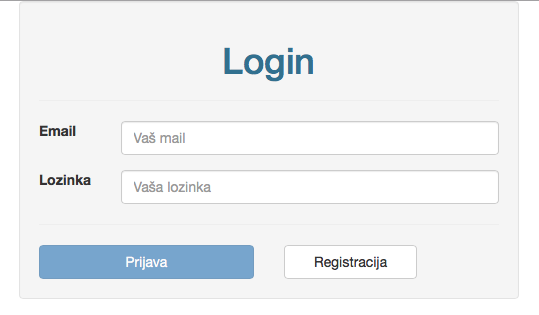
\includegraphics[width=0.5\textwidth]{login}
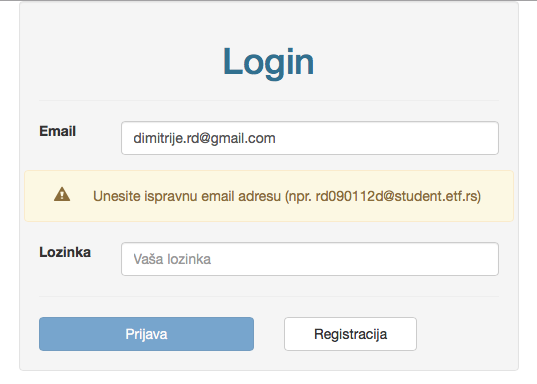
\includegraphics[width=0.5\textwidth]{login-wrongemail}
\caption{Levo: inicijalni izgled login stranice, desno: login stranica tokom unosa email adrese}
\label{fig:login}
\end{figure}
Pokušaj prijave korisnika koji nije registrovan, ili koji se ulogovao sa pogrešnom lozinkom se prikazuju kao greška (slika \ref{fig:login-error}).
\begin{figure}[p]
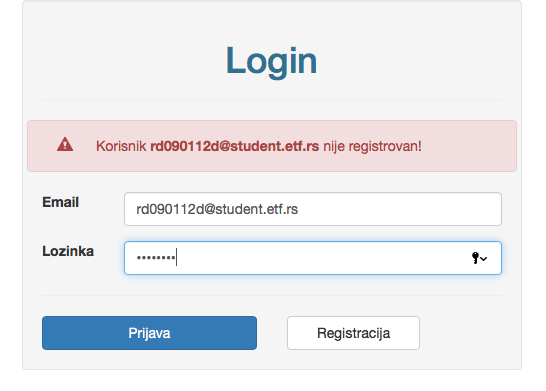
\includegraphics[width=0.5\textwidth]{login-error-unknown}
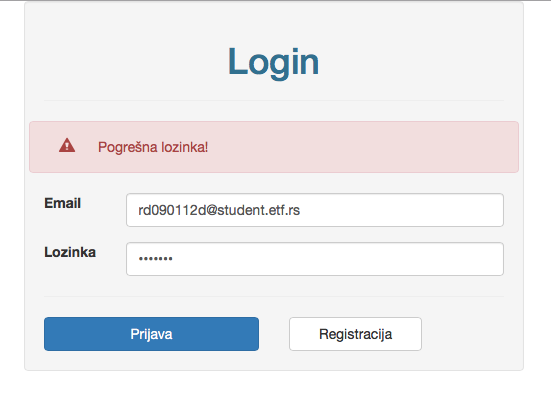
\includegraphics[width=0.5\textwidth]{login-error-password}
\caption{Login stranica nakon što neregistrovani korisnik pokuša da se uloguje (levo), ili ukoliko korisnik unese pogrešnu lozinku (desno)}
\label{fig:login-error}
\end{figure}

Novi korisnici mogu da se registruju pritiskom na dugme \textbf{Registracija}. Ta akcija ih vodi na stranicu za registrovanje novih korisnika (slika \ref{fig:register}), koja od korisnika traži da unese email adresu (ista ograničenja vezana za email adresu se primenjuju i ovde). Pokušaj postojećeg korisnika da se ponovo registruje rezultuje greškom. Nakon što unese email, pritiskom na dugme \textbf{Izvrši} se korisnik registruje na sistem. Nakon uspešne registracije korisniku se prikazuje stranica sa slike \ref{fig:register-success}. Tom prilikom se na unetu email adresu automatski šalje email sa nasumično generisanom lozinkom za tog korisnika. Sa ovom lozinkom korisnik sada može da se uloguje na sistem preko stranice za logovanje.
\begin{figure}[p]
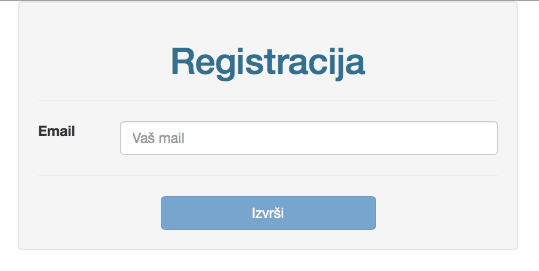
\includegraphics[width=0.5\textwidth]{register}
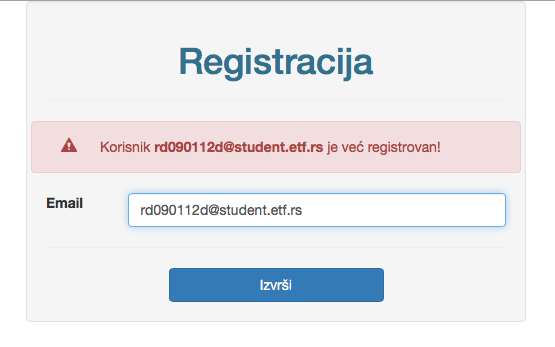
\includegraphics[width=0.5\textwidth]{register-error}
\caption{\textit{Levo}: inicijalni izgled stranice za registrovanje, \textit{desno}: stranica za registracije nakon što već registrovani korisnik pokuša da se registruje}
\label{fig:register}
\end{figure}
\begin{figure}[h]

\includegraphics[width=\textwidth]{register-success}
\caption{Izgled stranice za registraciju nakon uspešne registracije}
\label{fig:register-success}
\end{figure}

\subsection{Stranica sa pregledom testova}
Nakon uspešne prijave na sistem, korisniku se prikazuje stranica sa pregledom svih testova trenutno u sistemu. Ova stranica se prikazuje i kao početna stranica ukoliko je korisnik već ulogovan na sistem, a pregledač usmeri na \textit{root} URL servisa. Testovi su grupisani po kategorijama, i prikazani unutar tabele u svakoj kategoriji. Za svaki test se prikazuje ime testa, broj stranica sa pitanjima, i ukupan broj pitanja. Testovi koji se prikazuju na ovoj stranici se dele na:
\begin{itemize}
\renewcommand\labelitemi{--}
\item \textbf{Završene testove}, tj. testove koje je korisnik predao. Za ove testove se dodatno prikazuju datum i vreme kada je test započet, datum i vreme kada je test završen, procenat od ukupnog broja pitanja na koja je student dao odgovor, tj. progres, i najzad ocena, u vidu procenta tačnih odgovora u odnosu na ukupan broj pitanja. Boja pozadine ovih unosa je zelena.
\item \textbf{Testove u toku}, tj. testove koje je korisnik započeo, ali nije završio. Za ove testove se dodatno prikazuju datum i vreme kada je test započet, progres, i link ka stranici sa testom. Boja pozadine ovih unosa je žuta.
\item \textbf{Nezapočete testove}, tj. testove koje korisnik nikada nije polagao. Za ove testove se dodatno prikazuje link ka stranici sa testom. Boja pozadine ovih unosa je bela.
\end{itemize}
